\chapterimage{09_Snov.jpg} % Chapter heading image

\chapter{Interakcija svetlobe s snovjo}
V tem poglavju bomo podrobneje obravnavali interakcijo svetlobe s snovjo, ki jo 
v najpreprostejši obliki opišemo z lomnim količnikom. Na poenostavljenem modelu
bomo spoznali odvisnost lomnega količnika od frekvence vpadnega valovanja in pojasnili
posledice disperzije. Zapisali bomo tudi lomni količni za prevodne snovi ter
opisali dva zanimiva pojava: optično aktivnost in Faradayev pojav.

\section{Fazna in grupna hitrost}
V tretjem poglavju smo zapisali osnovno rešitev valovne enačbe
v neomejenem prostoru (enačba~\ref{eq:valovnaE}) v obliki ravnih valov 
(enačba~\ref{eq:ravnival}). Izračunali smo fazno hitrost,
to je hitrost premikanja ploskev konstantne faze oziroma valovnih front, in
jo zapisali kot razmerje krožne frekvence vpadne svetlobe 
in valovnega števila (enačba~\ref{eq:03_10}):
\boxeq{eq:09_25a}{
v_f = \frac{\omega}{k}
}
Fazno hitrost svetlobe navadno označimo s $c$ in jo zapišemo kot (enačba~\ref{eq:c}):
\beq
c = \frac{c_0}{n}.
\label{eq:09_01}
\eeq
Pri tem lomni količnik $n$ označuje razmerje med hitrostjo svetlobe v 
vakuumu $c_0$ in hitrostjo svetlobe v snovi $c$. Na splošno je lomni količnik odvisen 
od snovi, po kateri se svetloba širi, in tudi od frekvence vpadne svetlobe.

Obravnavajmo dve ravni valovanji z enakima amplitudama $E_0$, ki potujeta v isti smeri vzdolž
osi~$z$. Njuni frekvenci naj se le malo razlikujeta, zato ju zapišimo kot: 
$\omega_1=\omega + \Delta \omega$ in $\omega_2=\omega - \Delta \omega$, pripadajoči
valovni števili naj bosta: $k_1 = k + \Delta k $ in $k_2 = k - \Delta k$. 
Vsoto teh dveh valovanj zapišemo kot:
\begin{align}
E &= E_0 \cos (k_1z-\omega_1 t)+ E_0 \cos (k_2z-\omega_2 t) \nonumber\\
&= E_0 \cos\left((k+\Delta k)z-(\omega + \Delta \omega)t\right) 
+ E_0 \cos\left((k-\Delta k)z-(\omega - \Delta \omega)t\right)\nonumber \\
&= E_0 \cos\left((kz - \omega t) +(\Delta k z-\Delta \omega t\right)
+ E_0 \cos\left((k z - \omega t) - (\Delta k z- \Delta \omega t)  \right)\!. 
\label{eq:09_23}
\end{align}
Z uporabo adicijskega izreka za kotne funkcije:
\beq
\cos\alpha + \cos \beta = 2 \cos \frac{\alpha + \beta}{2} \cos \frac{\alpha - \beta}{2}
\eeq
izraz preoblikujemo v:
\beq
E = 2\cos \left(kz - \omega t \right)\cos \left(\Delta kz - \Delta \omega t \right)\!.
\label{eq:09_24}
\eeq
Vsota teh dveh valovanj je torej potujoče valovanje v smeri $z$ s frekvenco, ki je 
enaka osrednji krožni frekvenci $\omega$, in valovnim številom, ki je enako 
osrednjemu valovnemu števiku $k$. Valovanje je amplitudno modulirano 
s krožno frekvenco $\Delta \omega$ (slika~\ref{fig:09_utripanje}).
\begin{figure}[ht]
\centering
\def\svgwidth{140truemm} 
\input{slike/09_vsota.pdf_tex}
\caption{Dve valovanji z različnimi frekvencami (modra in zelena, levo) se seštejeta
v amplitudno modulirano valovanje (desno).}
\label{fig:09_utripanje}
\end{figure}

Pri valovanju, ki predstavlja zaporedje potujočih sunkov, lahko določimo dve
različni hitrosti. Prva je hitrost premikanja ploskev konstantne
faze oziroma premikanja vrhov hitre modulacije. Ta hitrost je fazna hitrost in
jo izračunamo iz znane enačbe~(\ref{eq:09_25a}). Druga hitrost pa je hitrost, s katero
se premikajo vrhovi počasne modulacije oziroma posamezni sunki. Izračunamo jo
iz enačbe~(\ref{eq:09_24}) in dobimo 
\beq
v_g=\frac{z}{t} = \frac{\Delta \omega}{\Delta k}.
\eeq
Hitrost premikanja sunkov imenujemo grupna hitrost in jo 
v limiti majhnih frekvenčnih razlik zapišemo kot:
\boxeq{eq:09_24a}{
v_g = \frac{d\omega}{d k}.
}

Izraz za grupno hitrost smo sicer izpeljali na primeru valovanja, sestavljenega iz dveh
valovanj, vendar velja na splošno za razširjanje sunkov svetlobe. Informacija,
ki jo prenašajo sunki svetlobe, po snovi torej potuje z grupno hitrostjo.
\vglue5truemm
\begin{figure}[ht]
\centering
\def\svgwidth{130truemm} 
\input{slike/09_disperzija2.pdf_tex}
\caption{Posnetki potujočega amplitudno moduliranega valovanja ob različnih časih.
Potovanje posameznega vala označuje zelena pika, ki se premika z fazno hitrostjo. Potovanje
amplitudne modulacije označuje modra pika in ta se premika z grupno 
hitrostjo. Vidimo, da sta v narisanem primeru fazna in grupna hitrost različni.}
\label{fig:09_disperzija}
\end{figure}

Vstavimo zvezo med valovnim številom in krožno frekvenco $k=\omega n /c_0$ v izraz za 
grupno hitrost (enačba~\ref{eq:09_24a}) in dobimo:
\beq
v_g = \frac{d\omega}{dk } = \left(\frac{dk}{d\omega}\right)^{-1} = \left( \frac{d}{d\omega}\left( 
\frac{\omega n }{c_0}\right)\!\right)^{-1}\!\!.
\label{eq:09_25}
\eeq
Upoštevamo, da je lomni količnik na splošno odvisen od frekvence valovanja, in zapišemo:
\beq
v_g = \left(\frac{n}{c_0} + \frac{\omega}{c_0 }\frac{dn}{d\omega}\right)^{-1} = 
\frac{c_0}{n+\omega \frac{dn}{d\omega}}.
\label{eq:09_26}
\eeq
V zapisanem izrazu za grupno hitrost nastopa odvod lomnega količnika po krožni frekvenci vpadnega
valovanja. Če je lomni količnik konstanten in neodvisen od frekvence, je odvod enak nič in 
takrat sta fazna in grupna hitrost enaki. Na splošno je odvod različen od nič in v naslednjem razdelku
spoznali, da je za večino snovi odvod na celotnem spektralnem območju vidne svetlobe pozitiven.
Na splošno zato velja, da je za vidno svetlobo grupna hitrost manjša od fazne.

\section{Lomni količnik}
Odvisnost lomnega količnika od frekvence vpadnega 
elektromagnetnega valovanja bomo izračunali na preprostem modelu. 
Omejimo se na nemagnetne snovi, za katere je $\mu = 1$, kar pomeni, da
za izračun frekvenčne odvisnosti lomnega količnika zadošča poznati 
$\varepsilon(\omega)$. 

Naj bo snov sestavljena iz $N$
identičnih atomov oziroma molekul, ki so enakomerno porazdeljeni
po prostoru s prostornino $V$. Za opis posameznega atoma ali molekule uporabimo 
klasični model oscilatorja, ki ga imenujemo Lorentzov model 
po nizozemskem fiziku Hendriku Lorentzu (1853--1928). 

Zamislimo si, da atom oziroma molekulo sestavljata kroglica 
pozitivnega naboja, ki miruje v izhodišču pri $x=0$, in kroglica
(oblak) negativnega naboja na neki ravnovesni oddaljenosti. Med njima naj 
deluje privlačna sila, ki jo v klasičnem modelu opišemo z vzmetjo
s konstanto vzmeti $k$. 
Poleg elastične sile naj na negativno nabito kroglico med 
premikanjem deluje tudi sila dušenja, ki opisuje absorpcijo svetlobe
v snovi. V klasični sliki si lahko
zamislimo, da je ravnovesna razdalja med kroglicama enaka $x_r$, 
v bolj realističnem modelu, v katerem elektron opišemo kot oblak okoli jedra,
pa je ravnovesna razdalja enaka 0. Podobno velja tudi za molekule, ki 
nimajo dipolnega momenta. Ker je razlika le v konstanti, 
to na končni rezultat ne vpliva.
\begin{figure}[ht]
\centering
\def\svgwidth{60truemm} 
\input{slike/09_Lorentz.pdf_tex}
\caption{Preprost Lorentzov model atoma. Zaradi vpadnega 
elektromagnetnega valovanja elektron vzbujeno niha.
}
\label{fig:09_Lorentz}
\vglue-5truemm
\end{figure}

Naj na tak model atoma ali molekule vpada elektromagnetno valovanje. Ker je 
valovna dolžina svetlobe bistveno večja od atoma, lahko privzamemo, da
je električno polje po velikosti znotraj celotnega atoma homogeno in enako $E$.
Za negativno nabito kroglico (elektron) zapišemo Newtonov zakon, pri čemer upoštevamo silo vzmeti, silo 
dušenja in silo v električnem polju. Omejimo se na polarizacijo 
polja v smeri $x$ in zapišemo:
\beq
m \ddot{x} = -kx -\gamma m \dot{x} - e_0 E.
\label{eq:09_02}
\eeq
Pri tem so $m$ masa negativno nabite kroglice, $\gamma$ koeficient dušenja
in $E = E_0\,e^{-i\omega t}$.

\begin{remark}
Pri zapisu Lorentzovega modela smo privzeli, da je elektično polje, 
ki ga čuti atom, enako vpadnemu električnemu polju. 
To velja, dokler je atom sam oziroma snov sestavlja redek plin. Če je 
atom v snovi obdan z ostalimi atomi, 
čuti tudi njihov vpliv in pravilno bi bilo upoštevati skupni vpliv, ki 
ga zapišemo s tako imenovanim lokalnim poljem. 
Kako izračunamo lokalno polje, bomo spoznali v naslednjem razdelku. 
\end{remark}

Vpeljemo lastno krožno frekvenco $\omega_0 = k/m$ in 
enačbo prepišemo v:
\beq
\ddot{x} + \gamma \dot{x} + \omega_0^2 x  = - \frac{e_0}{m} E_0 e^{-i \omega t}.
\label{eq:09_04}
\eeq
Rešujemo jo z nastavkom:
\beq
x(t) = x_0 e^{-i\omega t},
\label{eq:09_05}
\eeq
pri čemer $x_0$ opisuje amplitudo nihanja, odvisno od $\omega$. Vstavimo nastavek 
(enačba~\ref{eq:09_05}) v enačbo~(\ref{eq:09_04}) in dobimo:
\beq
-\omega^2 x_0 - i \omega \gamma x_0 + \omega_0^2 x_0  = - \frac{e_0}{m} E_0.
\label{eq:09_06}
\eeq
Od tod izrazimo amplitudo nihanja v odvisnosti od frekvence vpadnega valovanja:
\beq
x_0 = \frac{-e_0/m~E_0}{\omega_0^2 - \omega^2 - i\gamma \omega}.
\label{eq:09_07}
\eeq
V zapisanem izrazu prepoznamo značilno resonančno odvisnost dušenega nihala. 

Vpadno električno polje izmakne negativno nabito kroglico iz ravnovesne 
lege, kar povzroči nastanek dipolnega momenta $\mathbf{p}$:
\beq
\mathbf{p} = -e_0\,x\,\mathbf{e}_x.
\label{eq:09_08}
\eeq
Prehod iz mikroskopskega opisa z dipolnim momentom posameznega atoma 
v makroskopski opis naredimo z upoštevanjem gostote atomov v snovi 
$\varrho = N/V$. Vpeljemo inducirano električno polarizacijo $\mathbf{P}$, ki 
je enaka celotnemu dipolnemu momentu na enoto volumna:
\beq
\mathbf{P} = \frac{\mathbf{p}N}{V} = \mathbf{p}\,\varrho. 
\label{eq:09_09}
\eeq
Z upoštevanjem enačb~(\ref{eq:09_07} in \ref{eq:09_08}) zapišemo 
električno polarizacijo v snovi kot:
\beq
\mathbf{P} = -e_0\,x\,\mathbf{e}_x\,\varrho = \frac{e_0^2\,\varrho/m}{\omega_0^2 
- \omega^2 - i\gamma \omega}\,\mathbf{e}_x\,E_0\,e^{-i\omega t}.
\label{eq:09_10}
\eeq
Spomnimo se, da lahko inducirano električno polarizacijo izrazimo z jakostjo
električnega polja v snovi:
\beq
\mathbf{P} = \varepsilon_0 (\epsilon-1) \mathbf{E}.
\label{eq:09_12}
\eeq
\vglue-5truemm
\begin{remark}
Gornji zapis je linearni približek zveze med električno polarizacijo in 
jakostjo električnega polja. Pri velikih vpadnih jakostih električnega polja linearna zveza 
ne velja in treba je upoštevati tudi višje člene v razvoju z višjimi potencami polja. Ti
opisujejo nelinearne optične pojave, kar presega okvir te knjige.
\end{remark}

Enačbo~(\ref{eq:09_12}) primerjamo z enačbo~(\ref{eq:09_10}) in dobimo:
\beq
\varepsilon= 1 + \frac{e_0^2\,\varrho/\varepsilon_0 m}{\omega_0^2 - \omega^2 - i\gamma \omega}.
\label{eq:09_13}
\eeq
Vpeljemo še tako imenovano plazemsko frekvenco:
\beq
\omega_p = \sqrt{\frac{e_0^2\,\varrho }{\varepsilon_0 m}}
\label{eq:09_14}
\eeq
in upoštevamo zvezo med dielektričnostjo in na splošno kompleksnim lomnim količnikom:
\beq
\varepsilon = \mathcal{N}^2.
\label{eq:09_15}
\eeq
Dobimo:
\boxeq{eq:09_16}{
\varepsilon = \mathcal{N}^2 = 1+ \frac{\omega_p^2}{\omega_0^2 - \omega^2 - i\gamma \omega}.
}
\begin{remark}
V plazmi se elektroni prosto gibljejo in niso vezani na atome,
zato za opis elektronov v plazmi velja $k=0$ in $\gamma = 0$. Za opis njihovega
gibanja ostane le še krožna frekvenca $\omega_p$, od tod ime plazemska frekvenca.
\end{remark}

Kompleksni lomni količnik $\mathcal{N}$ razdelimo na realni $n'$ in imaginarni del $n''$ in 
zapišemo:
\beq
\mathcal{N}^2 = (n'+in'')^2 = n'^2-n''^2+2in'n'' =  1+ \frac{\omega_p^2}{\omega_0^2 - \omega^2 - i\gamma \omega}.
\label{eq:09_17}
\eeq
Izenačimo realni in imaginarni del leve in desne strani enačbe in dobimo:
\beq
n'^2 -n''^2 = \varepsilon' = 1 + \frac{\left(\omega_0^2 - \omega^2\right)\omega_p^2}{\left(\omega_0^2 - 
\omega^2\right)^2 + \gamma^2 \omega^2}
\label{eq:09_18}
\eeq
ter 
\beq
2n'n'' = \varepsilon'' = \frac{\gamma \omega \omega_p^2}{\left(\omega_0^2 - 
\omega^2\right)^2 + \gamma^2 \omega^2}.
\label{eq:09_19}
\eeq
Zapisali smo sistem dveh enačb za realni in imaginarni del lomnega količnika. Rešujemo ga podobno kot
sistem enačb za lomni količnik v prevodni snovi (enačbe~\ref{eq:nkompleks2} in \ref{eq:03_72})
z rešitvami v obliki enačb~(\ref{eq:03_76} in \ref{eq:03_77}). Rešitvi sta tako:
\beq
n'^2 = \frac{1}{2}\left(\varepsilon'+\sqrt{\varepsilon'^2 + \varepsilon''^2}\right)
\label{eq:09_20}
\eeq
in
\beq
n''^2 = \frac{1}{2}\left(-\varepsilon'+\sqrt{\varepsilon'^2 + \varepsilon''^2}\right)\!,
\label{eq:09_21}
\eeq
pri čemer sta $\varepsilon'$ in $\varepsilon''$ podana z enačbama~(\ref{eq:09_18} in \ref{eq:09_19}).
Realni in imaginarni del lomnega količnika sta tako odvisna od frekvence vpadnega valovanja. 
Odvisnost lomnega količnika od frekvence vpadnega elektromagnetnega valovanja, zaradi katere
se fazna in grupna hitrost valovanja v snovi razlikujeta, imenujemo disperzija.

\section{Disperzija}
Na preprostem modelu smo izpeljali lomni količnik snovi in pokazali,
kako se njegov realni in imaginarni del
spreminjata s frekvenco vpadnega elektromagnetnega valovanja. Ker so izrazi
razmeroma zapleteni, se navadno poslužimo približkov. Prvi naj 
bo približek redkega plina. 

V redkem plinu vrednost lomnega količnika le malo odstopa od lomnega količnika vakuuma 
in $\mathcal{N} \approx 1$. Lomni količnik (enačba~\ref{eq:09_17}) zato lahko razvijemo in dobimo:
\begin{align}
\mathcal{N} =& \sqrt{1+ \frac{\omega_p^2}{\omega_0^2 - \omega^2 - i\gamma \omega}} \\
\approx& 1 + \frac{1}{2}\frac{\left(\omega_0^2 - \omega^2\right)\omega_p^2}{\left(\omega_0^2 - 
\omega^2\right)^2 + \gamma^2 \omega^2} + \frac{i}{2}\frac{\gamma \omega \omega_p^2}{\left(\omega_0^2 - 
\omega^2\right)^2 + \gamma^2 \omega^2}.
\label{eq:09_22}
\end{align}
\begin{figure}[h!]
\centering
\def\svgwidth{140truemm} 
\input{slike/09_real_im_n.pdf_tex}
\caption{Odvisnost realnega (a) in imaginarnega dela (b) lomnega količnika od 
frekvence vpadne svetlobe v preprostem Lorentzovem modelu. Osenčen del na levi 
sliki označuje območje anomalne disperzije.}
\label{fig:09_nkompleks}
\end{figure}

Poglejmo najprej realni del lomnega količnika (slika~\ref{fig:09_nkompleks}\,a). 
Pri majhnih vrednostih je lomni količnik nekoliko večji od 1, 
njegova velikost pa je odvisna od razmerja med plazemsko in lastno frekvenco.
V bližini lastne frekvence $\omega_0$ lomni količnik naraste, nato strmo pade, potem pa 
začne ponovno naraščati in se počasi približuje vrednosti 1. V skoraj celotnem 
spektralnem območju je tako odvod lomnega količnika po frekvenci pozitiven 
(območje normalne disperzije), razen v ozkem območju v bližini lastne 
frekvence $\omega_0$, kjer je odvod negativen (območje anomalne disperzije). 
Za zelo velike frekvence vpadne svetlobe je lomni količnik praktično enak 1.

Izkaže se, da za praktično vse snovi lastna frekvenca $\omega_0$
leži v ultravijoličnem delu spektra, torej pri frekvencah, ki so večje od
frekvenc vidne svetlobe. Posledično je lomni količnik za vidno svetlobo 
vedno večji od 1. Za zelo velike frekvence, na primer za rentgensko svetlobo,
je lomni količnik manjši od 1. Lomni količnik kremena pri valovni 
dolžini $0,5~\si{nm}$ je tako $0,9998$. 

Odvod lomnega količnika po frekvenci vpadne svetlobe $dn/d\omega >0$
je za vse frekvence, razen v bližini $\omega_0$, pozitiven. 
Ker so frekvence vidne svetlobe manjše od lastnih frekvenc, je tudi celotna
vidna svetloba v območju normalne disperzije, kar pomeni, da z naraščajočo
frekvenco (in pojemajočo valovno dolžino) lomni količnik narašča. 
Po enačbi~(\ref{eq:09_26}) to pomeni, da je grupna hitrost vpadne vidne 
svetlobe vedno manjša od fazne hitrosti. 

Poglejmo še imaginarni del lomnega količnika (slika~\ref{fig:09_nkompleks}\,b), ki 
opisuje absorpcijo svetlobe. Večinoma je enak nič, razen v bližini lastne frekvence. 
V območju anomalne disperzije, v katerem je grupna hitrost večja od fazne, se 
torej vpadna svetloba močno absorbira. 

\begin{remark}
Vpadna svetloba se lahko absorbira zaradi različnih pojavov. To so lahko 
elektronski prehodi (tipično v vidnem ali ultravijoličnem delu spektra), 
vzbujanje vibracijskih stanj v snovi (infrardeč del spektra) ali 
vzbujanje rotacijskih stanj (v mikrovalovnem delu spektra).
\end{remark}

Disperzijo smo pojasnili na preprostem Lorentzovem modelu.
V dejanski snovi oziroma atomskem/molekulskem sistemu je navadno več resonanc, pri čemer
vsaki od njih ustrezata neka resonančna frekvenca $\omega_{0j}$ in koeficient
dušenja $\gamma_j$. Potem vse prispevke zapišemo kot vsoto posameznih prispevkov 
z ustreznimi amplitudami $f_j$:
\beq
\varepsilon = \mathcal{N}^2 = 1+ \sum_j \frac{f_j \omega_{pj}^2}{\omega_{0j}^2 - \omega^2 - i\gamma_j\omega}.
\label{eq:09_27}
\eeq
\begin{figure}[h!]
\centering
\def\svgwidth{140truemm} 
\input{slike/09_disp_multi.pdf_tex}
\caption{Primer disperzije realnega dela lomnega količnika za Lorentzov model 
z več lastnimi resonancami. Senčeni del označuje območje vidne svetlobe, 
za katero velja normalna disperzija.}
\label{fig:09_disp_multi}
\end{figure}

V praksi za navedeni izraz uporabimo različne približke, ki v danem frekvenčnem
območju dovolj dobro opišejo odvisnost lomnega količnika. V prozornih snoveh lahko 
dušenje, ki na splošno povzroča absorpcijo, povsem zanemarimo in privzamemo $\gamma_j = 0$ za 
vsak $j$. V tem približku dobimo:
\beq
\mathcal{N}^2 = n'^2 = 1+ \sum_j \frac{f_j \omega_{pj}^2}{\omega_{0j}^2 - \omega^2}.
\label{eq:09_28}
\eeq
Če namesto krožne frekvence vstavimo valovno dolžino svetlobe, dobimo:
\beq
n'^2 = 1 + \sum_j \frac{f_j \omega_{pj}^2\lambda_{oj}^2\lambda^2}{\lambda^2 - \lambda_{0j}^2}.
\label{eq:09_29}
\eeq
Kadar je valovna dolžina vpadne svetlobe razmeroma blizu eni lastni frekvenci in daleč
od ostalih, lahko prispevke ostalih lastnih frekvenc upoštevamo le v konstanti in ostane:
\boxeq{eq:09_30}{
n'^2(\lambda) = A + \sum_j \frac{G_j \lambda^2}{\lambda^2 - \lambda_{0j}^2}.
}
Približek je leta 1872 zapisal nemški fizik Wolfgang von Sellmeier, zato ga danes
imenujemo Sellmeierjeva enačba. Ta zveza se pogosto uporablja za opis disperzije 
lomenga količnika $n(\lambda)$ v prozornih snoveh. 

Še preprostejši približek je Cauchyjev približek, ki ga imenujemo po francoskem matematiku
Augustin-Louisu Cauchyju (1789--1857). Uporabimo ga lahko, kadar je izbrano spektralno
območje dovolj daleč od resonanc. Poleg tega upoštevamo, da se lomni količnik le malo 
razlikuje od 1, in zapišemo:
\boxeq{eq:09_30a}{
n = A + \frac{B}{\lambda^2}.
}

\begin{example}{\bf Cauchyjev približek za lomni količnik.}
Najpreprostejši opis odvisnosti lomnega količnika od valovne dolžine vpadne svetlobe
je Cauchyjev približek. Čeprav smo zvezo izračunali za redke pline, velja v vidnem
območju dovolj dobro tudi
za gostejše trdne snovi. Nekaj parametrov $A$ in $B$ za izračun lomnega količnika
je podanih v tabeli:
\begin{center}
\begin{tabular}{|l|l|l|}
\hline
snov& $A$ & $B (\si{\micro\metre}^2)$\\ \hline 
taljeno kremenovo steklo & 1,4580 & 0,00354\\ \hline
kronsko steklo K5 & 1,5220 & 0,00459\\ \hline
svinčevo steklo SF10 & 1,7280 & 0,01342\\ \hline
\end{tabular}
\end{center}
\end{example}

\subsection*{Popravek lokalnega polja v gosti snovi}
Do zdaj smo obravnavali redko snov, v kateri so atomi oziroma molekule
dovolj oddaljeni, da ne čutijo medsebojnega vpliva. 
Zato smo v preprostem Lorentzovem modelu za polje, ki ga čuti elektron, 
vzeli kar polje vpadne svetlobe $E$. Če pa je izbrana molekula obdana
z drugimi molekulami, ki se pod vplivom zunanjega električnega polja 
ravno tako polarizirajo, se  električno polje na mestu izbrane 
molekule spremeni. Za izračun tako imenovanega lokalnega polja $\tilde{E}$
moramo upoštevati tudi okoliško polarizacijo.

Lokalnega polja na tem mestu ne bomo izračunali (glej npr. Born in Wolf, {\it
Principles of Optics}), zapišimo le, da v izotropnih snoveh velja:
\beq
\tilde{E} = E + \frac{P}{3\varepsilon_0},
\label{eq:09_31}
\eeq
pri čemer smo se omejili le na eno smer, zato smo vektorski zapis opustili. 
Prvi člen v enačbi~(\ref{eq:09_31}) predstavlja jakost električnega 
polja vpadne svetlobe, drugi člen pa opisuje polarizacijsko 
polje zaradi okoliških molekul. Z uporabo zveze
$P = \varepsilon_0 (\varepsilon -1) E$ dobimo:
\beq
\tilde{E} = E + \frac{\varepsilon_0 (\varepsilon -1) E}{3\varepsilon_0} = 
\frac{\epsilon + 2}{3}E.
\label{eq:09_32}
\eeq
Jakost lokalnega polja je tako sorazmerna jakosti vpadnega polja. 

Pri izračunu inducirane polarizacije vseh dipolov v snovi (enačba~\ref{eq:09_10}) 
moramo zaradi vpliva sosednjih molekul upoštevati $\tilde{E}$. Sledi:
\beq
P = \frac{e_0^2\,\varrho/m}{\omega_0^2 - \omega^2 -i\gamma \omega}
\frac{\varepsilon+2}{3}\,E_0\,e^{-i\omega t}
= \varepsilon_0 (\varepsilon -1) E_0\,e^{-i\omega t}.
\label{eq:09_33}
\eeq
Od tod izračunamo zvezo:
\beq
\frac{\varepsilon -1 }{\varepsilon+2} = \frac{\mathcal{N}^2-1}{\mathcal{N}^2+2} = 
\frac{\omega_p^2/3}{\omega_0^2 - \omega^2 - i\gamma \omega}.
\label{eq:09_34}
\eeq
Če je krožna frekvenca vpadne svetlobe daleč od lastnih frekvenc, lahko dušenje zanemarimo in 
izraz preoblikujemo v:
\beq
\frac{\varepsilon -1 }{\varepsilon+2} = \frac{\mathcal{N}^2-1}{\mathcal{N}^2+2} = 
\frac{\omega_p^2}{3\left(\omega_0^2 - \omega^2\right)}.
\label{eq:09_35}
\eeq
Zapisani izraz imenujemo Lorentz-Lorenzova zveza po danskem matematiku Ludvigu Lorenzu 
(1829--1891) in nizozemskemu fiziku Hendriku Lorentzu. 
\begin{remark}
 Lorentz-Lorenzova zveza je tesno povezana s Clausius-Mossottijevo zvezo, ki opisuje
 zvezo med dielektrično konstanto snovi z atomsko polarizirnostjo $\alpha$:
 \beq
\frac{\varepsilon -1 }{\varepsilon+2} = \frac{\varrho\alpha}{3 \varepsilon_0},
\label{eq:09_35a}
\eeq
pri čemer je $\varrho$ število molekul na volumsko enoto. 
\end{remark}

\begin{example}{\bf Disperzija v steklu in v vodi.}
Verjetno najbolj poznana posledica disperzije v steklu je razklon bele svetlobe
na prizmi. S tem poskusom je Newton v drugi polovici sedemnajstega stoletja
pokazal, da je bela svetloba sestavljena iz svetlob različnih barv. Ko bela
svetloba vpade na prizmo, se lomi po lomnem zakonu. Ker je lomni kot odvisen
od valovne dolžine svetlobe, se svetloba različnih barv lomi pod različnimi
koti in ob izhodu iz prizme se snop prej bele svetlobe razkloni v različne
barve.
\begin{figure}[ht]
\centering
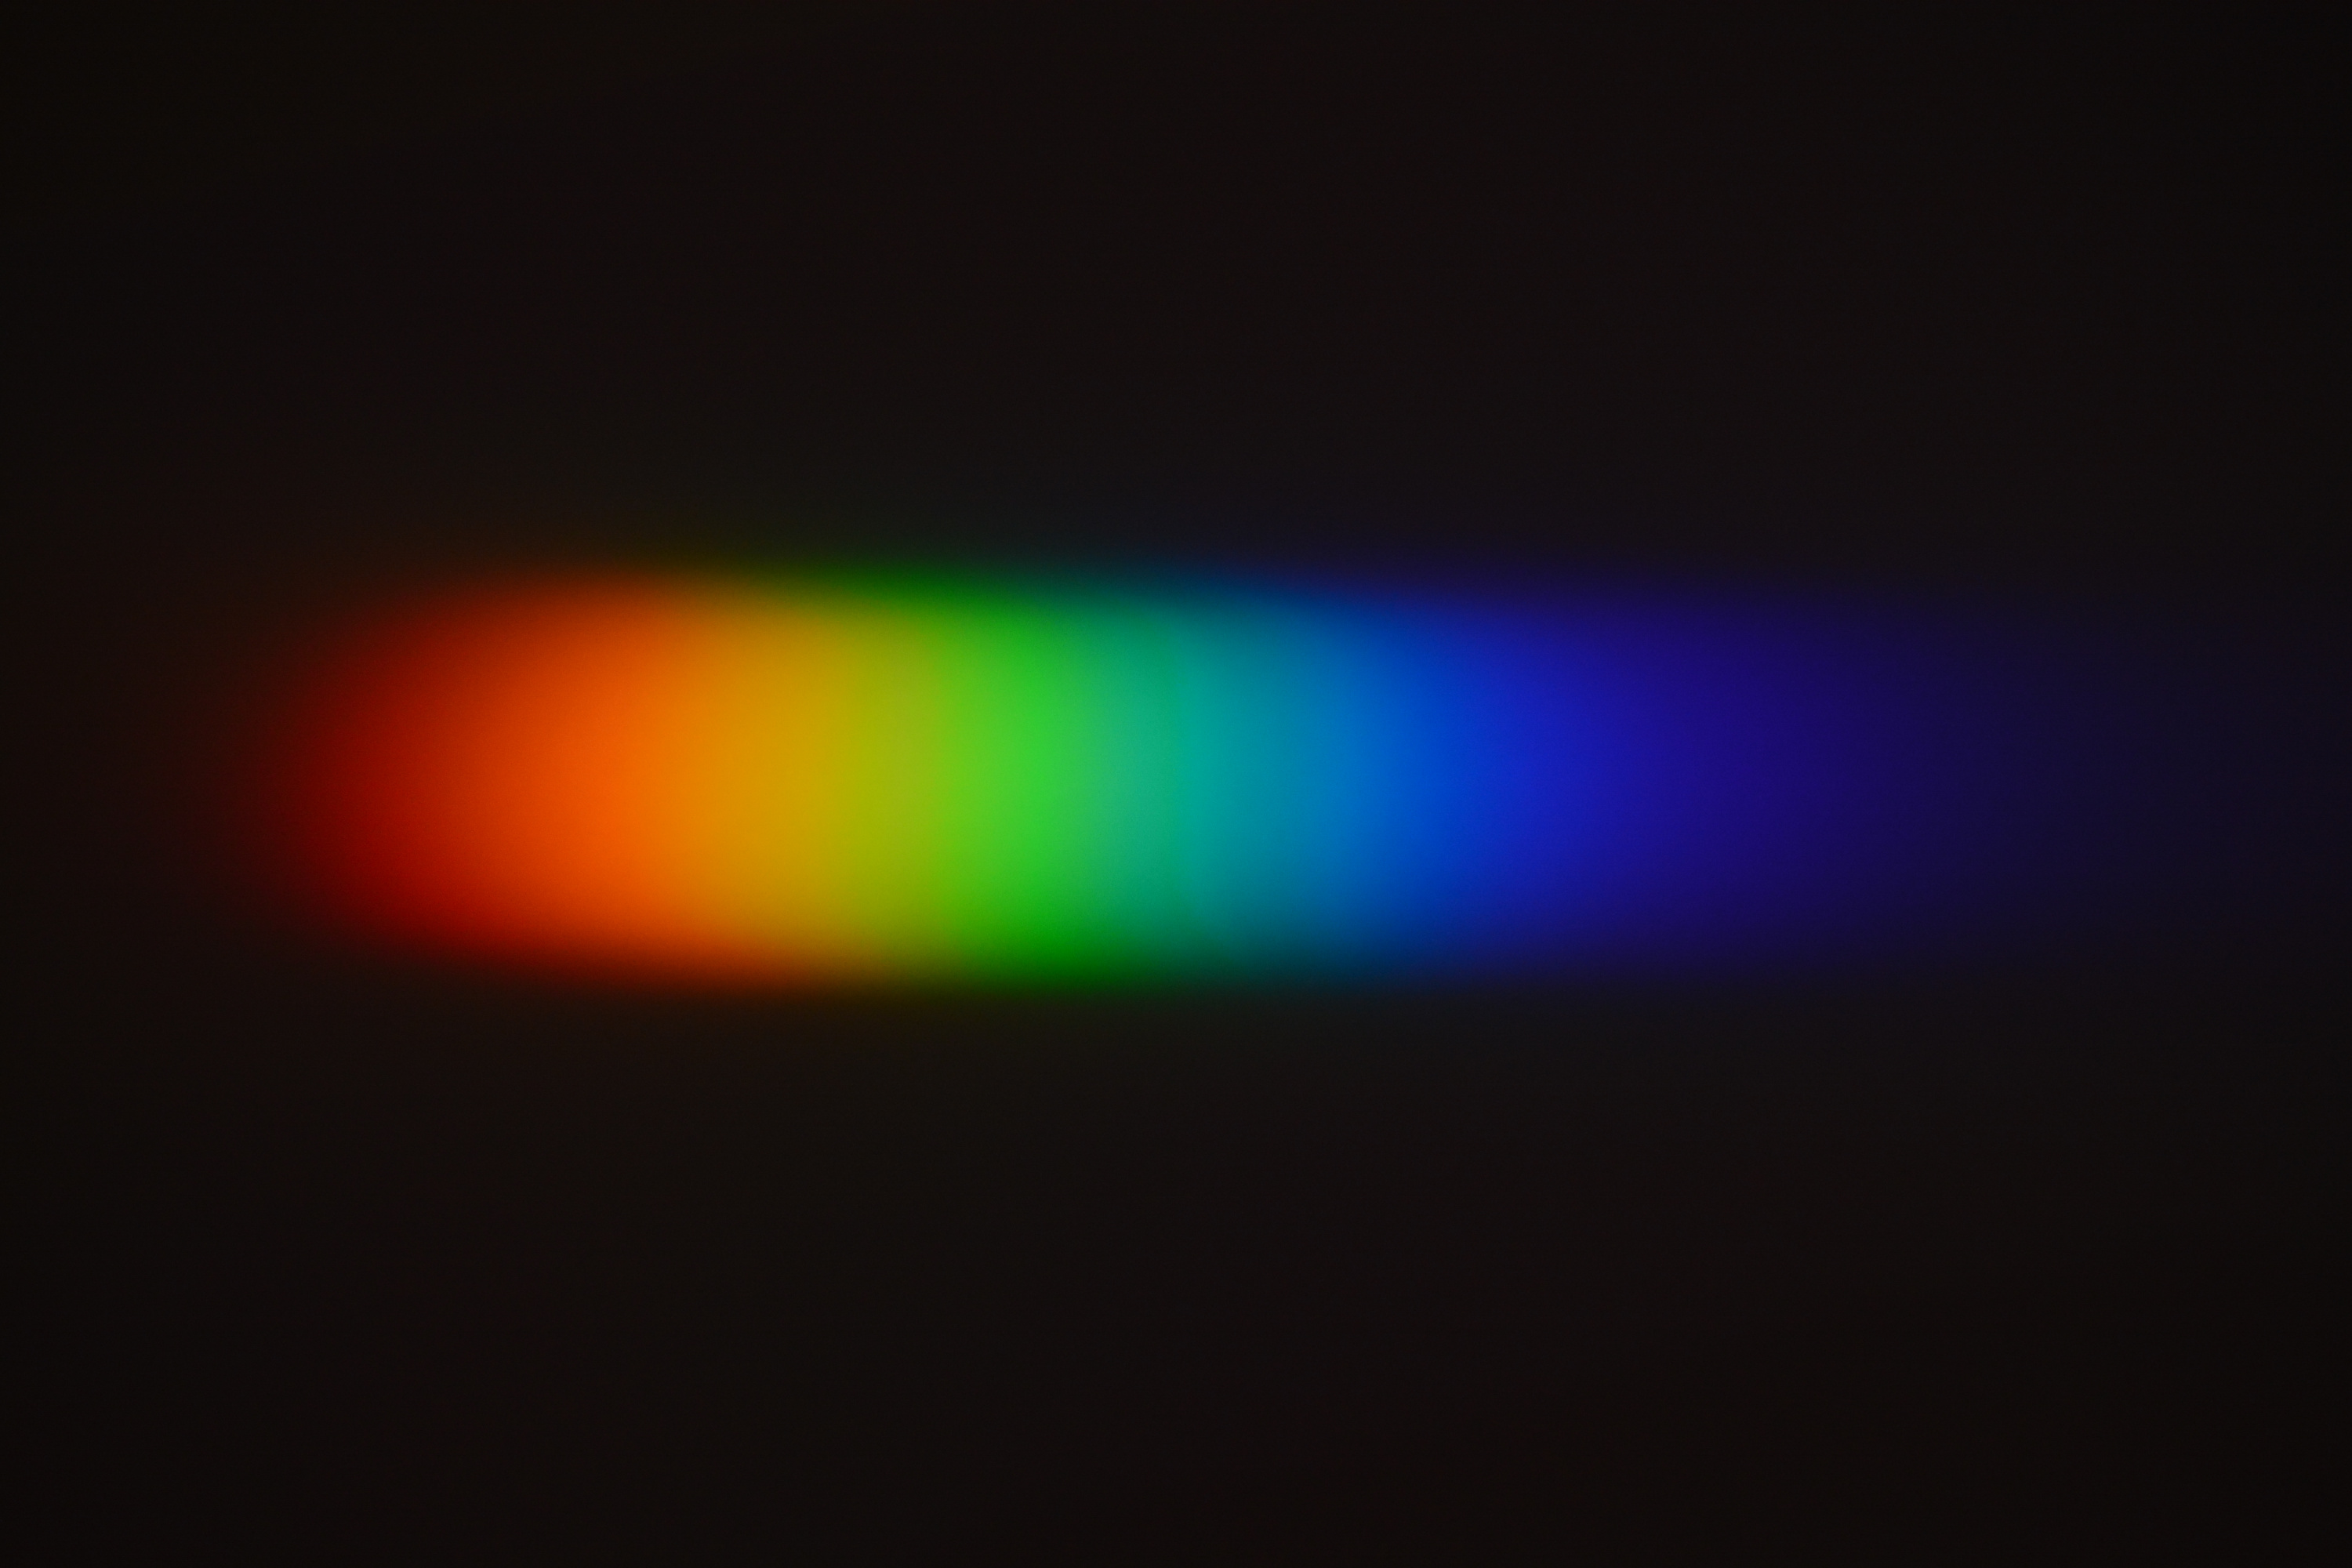
\includegraphics[width=7truecm]{slike/09_prizma.jpg}\hfill
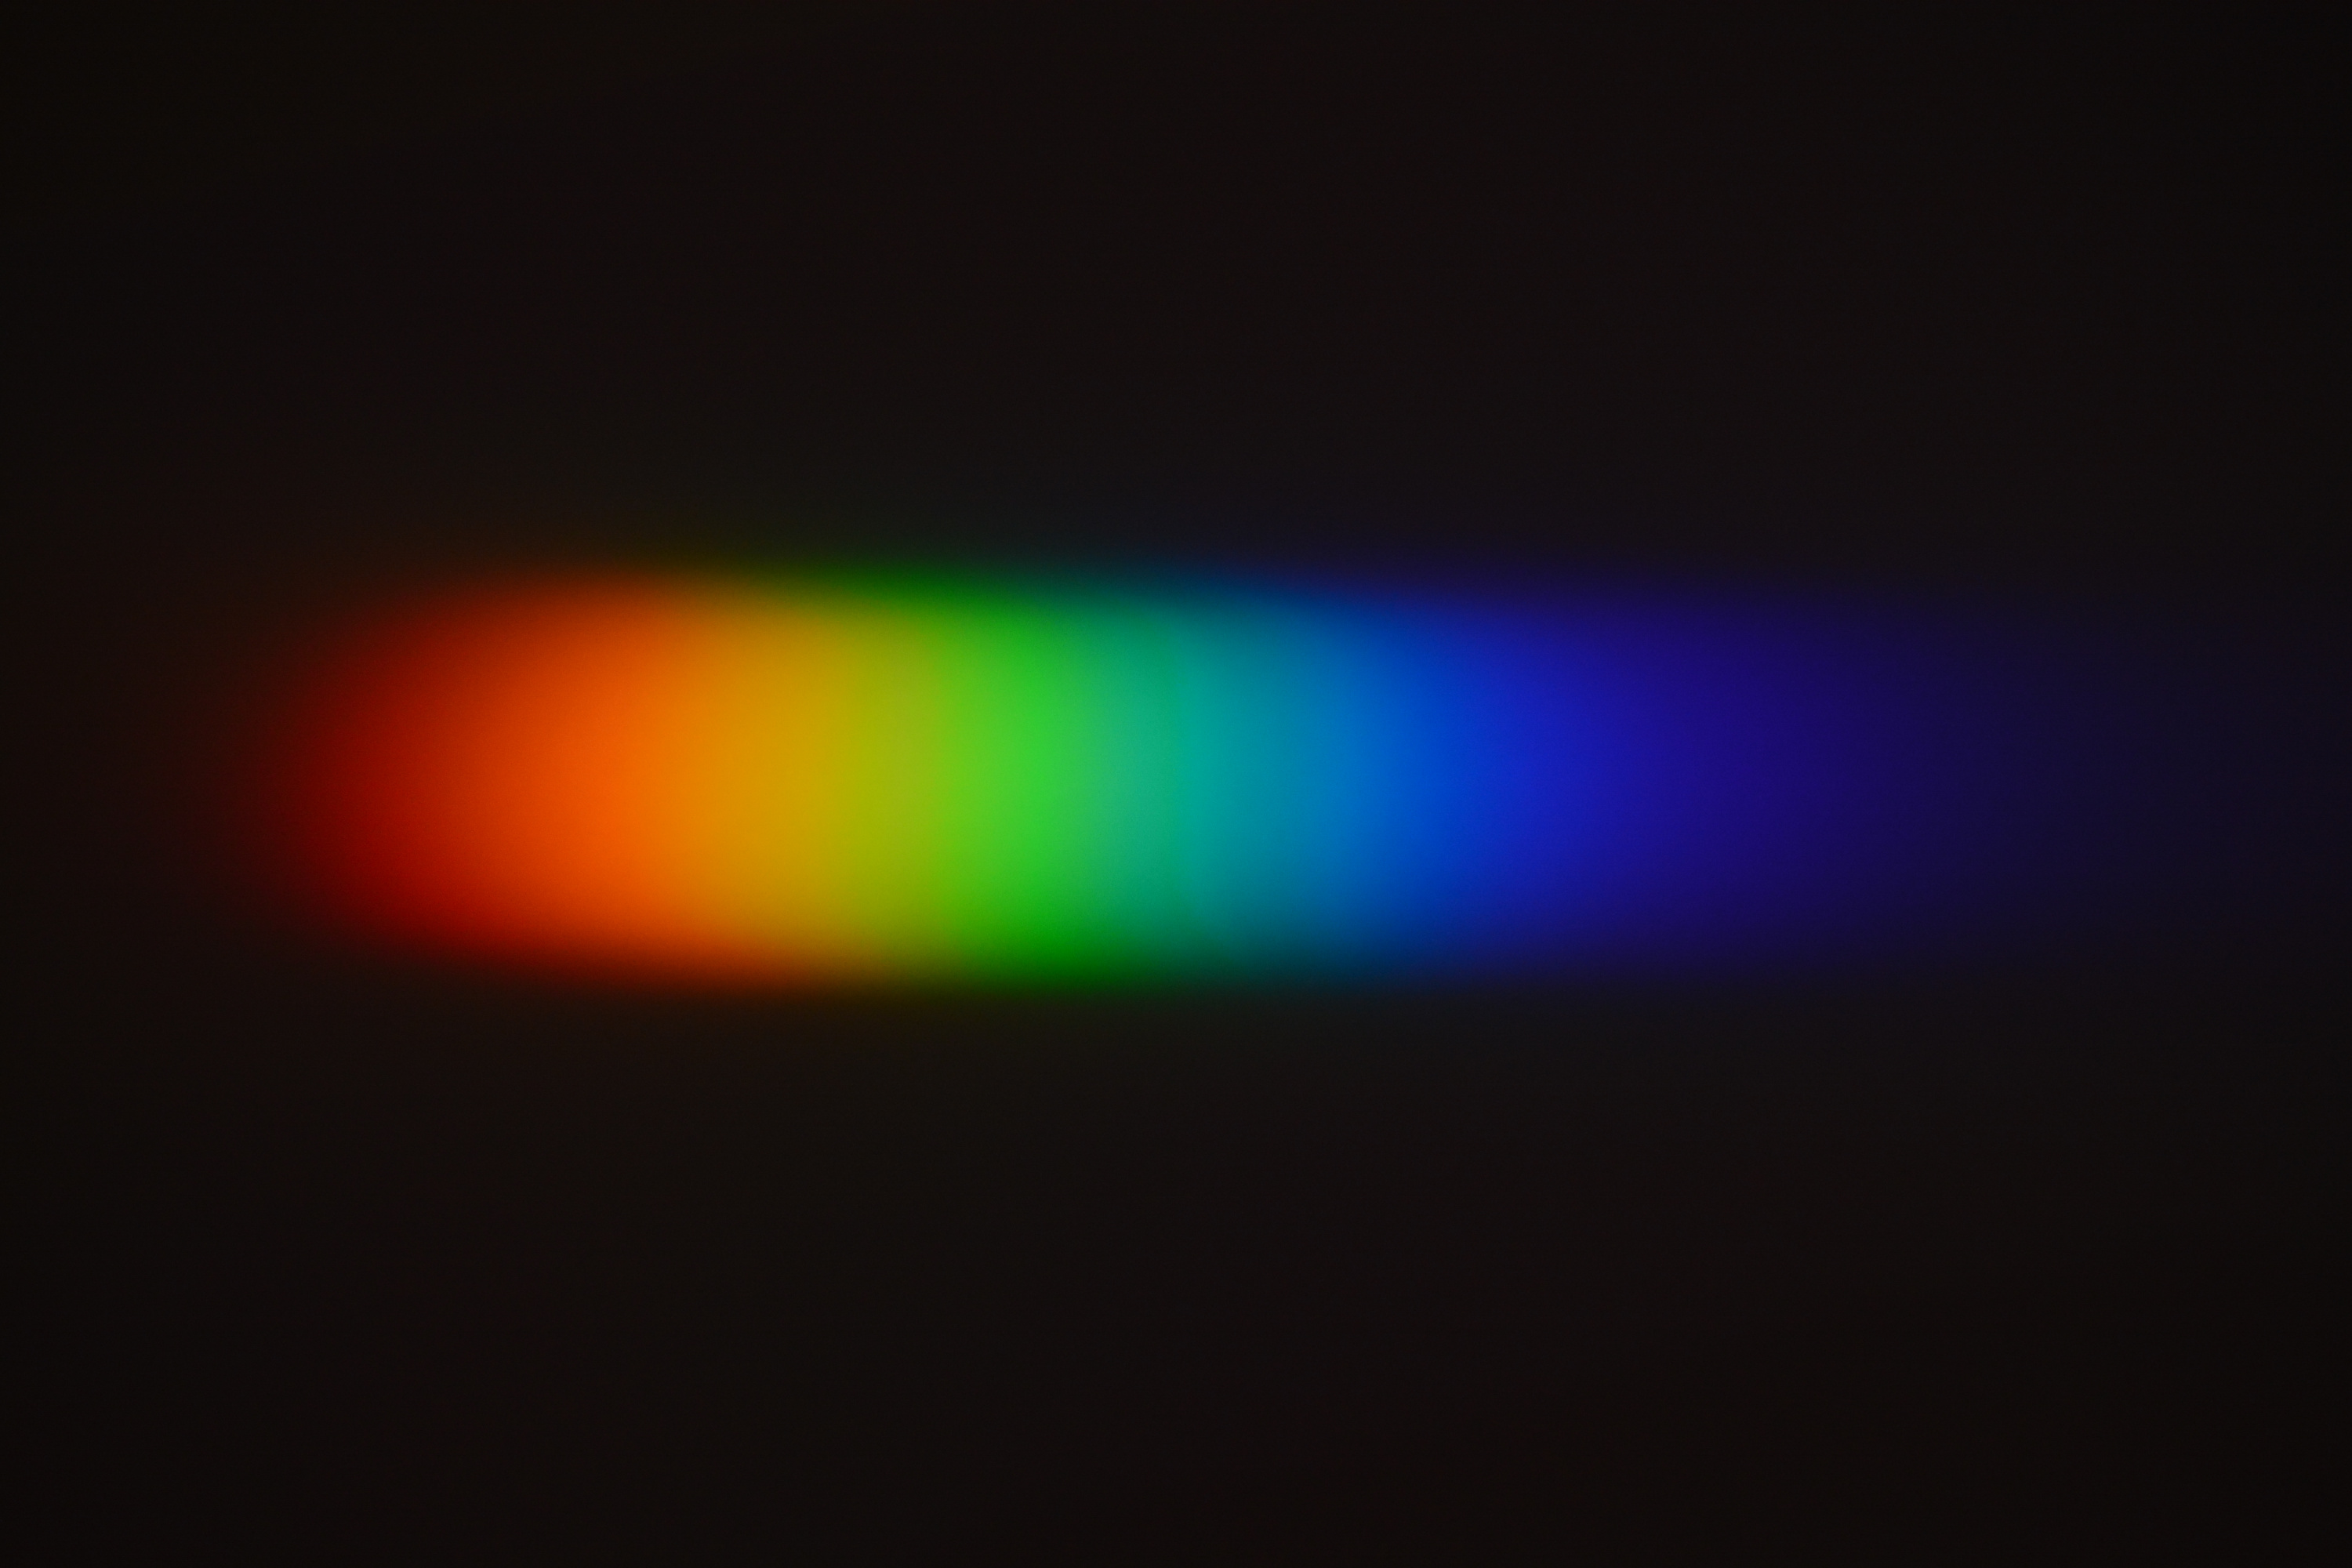
\includegraphics[width=7truecm]{slike/09_prizma.jpg}
\caption{Razklon sončne svetlobe na prizmi}
\label{fig:09_prizma}
\end{figure}
 
Drugi pomemben primer disperzije je mavrica, ki nastane zaradi
disperzije v dežnih kapljicah vode. Ko bela svetloba s Sonca vpade
na kapljice v zraku, se svetloba različnih valovnih dolžin 
lomi pod različnimi koti, in različne barve svetlobe izhajajo
iz kapljic pod različnimi koti. 
\begin{figure}[ht]
\centering
%\includegraphics[width=7truecm]{slike/09_mavrica_shema.jpg}\hfill
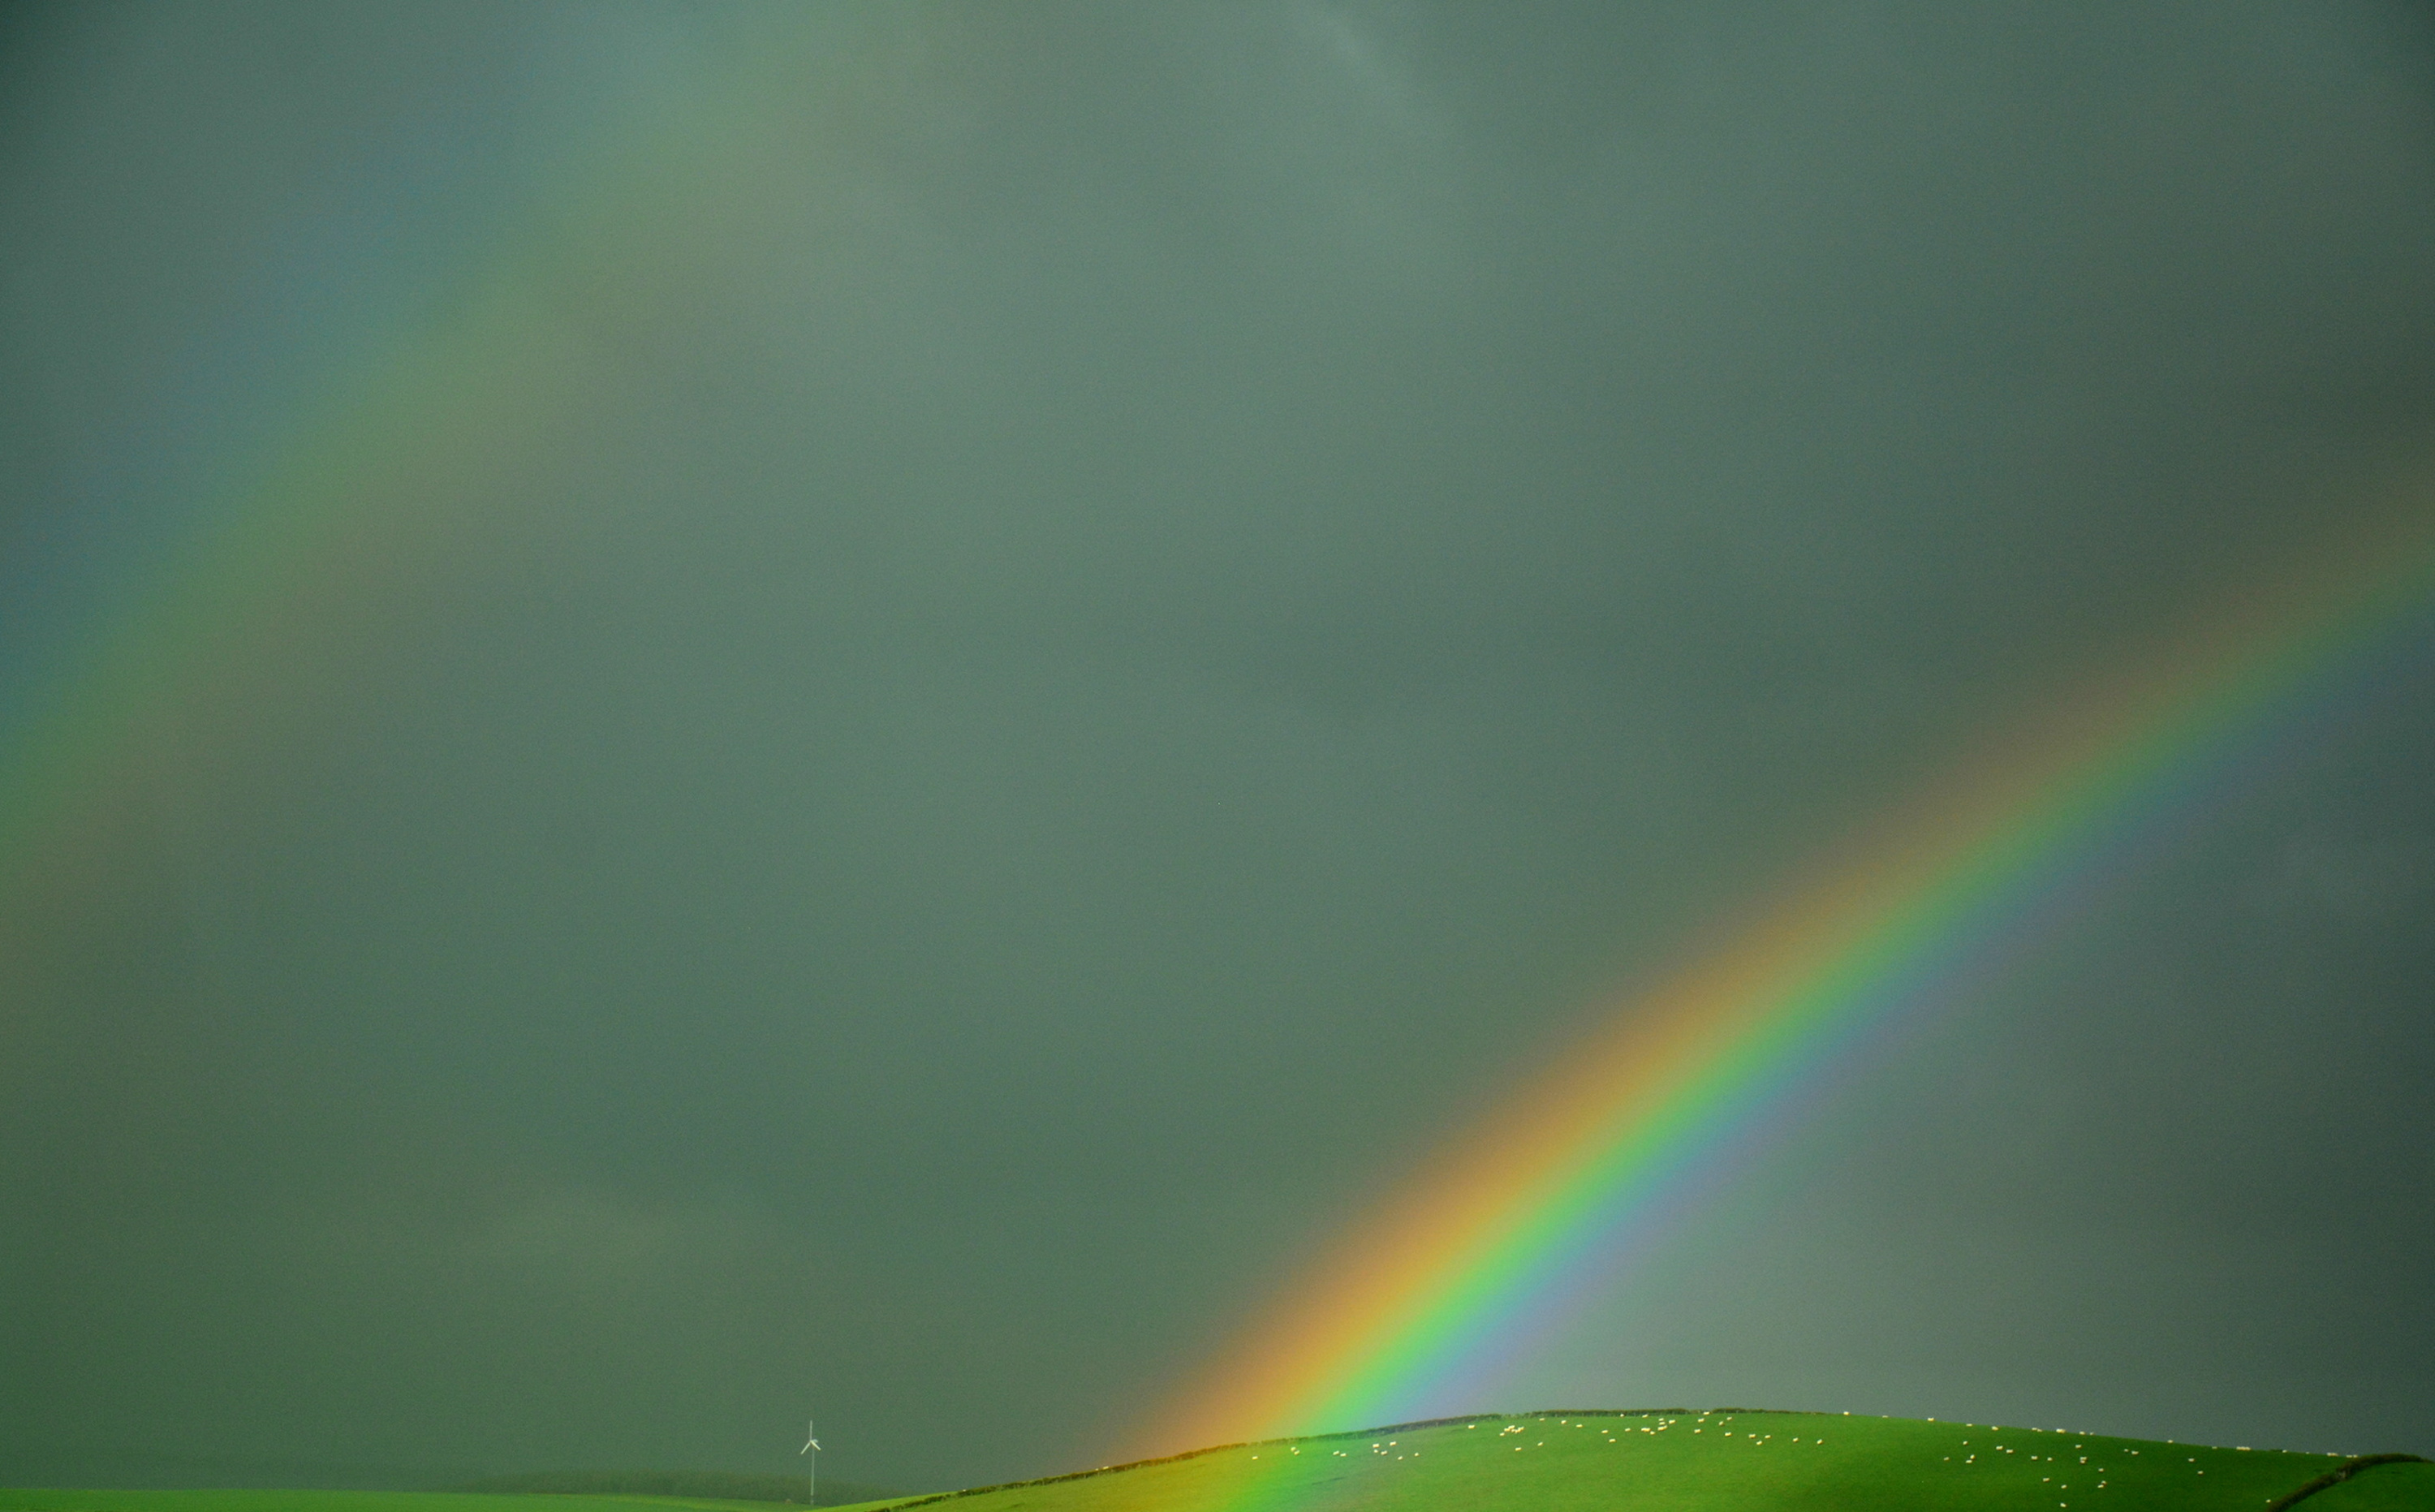
\includegraphics[width=7truecm]{slike/09_mavrica_photo.jpg}
\caption{Mavrica}
\label{fig:09_mavrica}
\end{figure}
\end{example}

\begin{example}{\bf Disperzija v optičnih vlaknih.}
Disperzija igra zelo pomembno vlogo pri prenosu signalov
po optičnih vlaknih. Informacija po vlaknih potuje
v obliki kratkih sunkov svetlobe, ki imajo neko
končno spektralno širino. Zaradi disperzije v vlaknih 
posamezne spektralne komponente sunka svetlobe
potujejo z malenkost različnimi hitrostmi, zaradi 
česar se sunek med prehodom skozi vlakno podaljša. 
Če so vpadni sunki svetlobe zelo kratki in si hitro sledijo,
se med prehodom skozi vlakno tako podaljšajo, da jih na izhodu
ne ločimo več in informacija se izgubi. 
Disperzija v optičnih vlaknih zato omejuje količino 
podatkov, ki jih lahko po vlaknu prenašamo v časovni enoti,
in veliko razvoja je posvečenega zmanjšanju disperzije.
\end{example}

\section{Prevodne snovi}
Elektrone v kovini obravnavamo po Drudejevem modelu prostega elektronskega plina
v mreži nepremičnih pozitivnih nabojev. Ker so v tem modelu elektroni prosti,
je konstanta vzmeti $k=0$ in tako lastna frekvenca $\omega_0=0$. Dobimo:
\beq
\mathcal{N}^2 = 1 + \frac{\omega_p^2}{-\omega^2 -i \gamma \omega} = 1- 
\frac{\omega_p^2}{\omega^2+i\gamma \omega}.
\label{eq:09_36}
\eeq
Če zanemarimo tudi električno upornost, ki ga opisuje koficient dušenja, dobimo
preprosto zvezo:
\beq
\mathcal{N} \approx \sqrt{1- \frac{\omega_p^2}{\omega^2}}.
\label{eq:09_37}
\eeq
Za vrednosti $\omega < \omega_p$ je lomni količnik povsem imaginaren in svetloba se v snovi
močno absorbira. Za krožne frekvence $\omega > \omega_p$ pa je lomni količnik realen 
in snov prozorna. 

Za na primer zlato je plazemska frekvenca pri okoli $500~\si{\nano\meter}$, v območju
vidne svetlobe torej, za srebro pa v ultravijoličnem območju pri okoli $320~\si{\nano\meter}$. 
Pri srebru je tako lomni količnik za celoten spekter vidne svetlobe imaginaren, zato se celoten 
spekter precej svetlobe enakomerno odbija. Pri zlatu je lomni količnik za del vidnega spektra realen in za
del vidnega spektra imaginaren. Rdeča in rumena barva se zato v snovi močno absorbirata, kar
je za zunanjega opazovalca videti, kot da se odbijeta. Modra svetloba v zlatu občuti
realni lomni količnik in se zato dosti manj odbija od površine kot rdeča in rumena. Ta
lastnost daje zlatu značilno rumeno-rdečkasto barvo. 


\section{Optični metamateriali}
Videli smo, da je v bližini resonanc ali v kovini pri $\omega <\omega_p$ vrednost $\mathcal{N}^2 <0$.
Lomni kolilčnik je zato povsem imaginaren. To se zgodi, ko je $\varepsilon'<0$. Dielektričnost
snovi ima negativno vrednost. Zanimive pojave dobimo, če hkrati velja tudi $\mu'<0$. Produkt
obeh je potem pozitiven in se lahko izognemo absorpciji. Vendar takrat velja drugačen
predznak za $\mathcal{N}$. Če denimo povsem zanemarimo dušenje ($\varepsilon''=0$, $\mu''=0$), 
potem velja $\varepsilon=\varepsilon'$ in $\mu  = \mu'$.
V navadnih snoveh velja:
\beq
\varepsilon >0, \mu > 0 \qquad \Rightarrow \qquad n^2 = \varepsilon \mu 
\qquad \Rightarrow \qquad n = \sqrt{\varepsilon\mu}. 
\label{eq:09_37m}
\eeq
Lahko pa velja tudi:
\beq
\varepsilon <0, \mu < 0 \qquad \Rightarrow \qquad n^2 = \varepsilon \mu 
\qquad \Rightarrow \qquad n = -\sqrt{\varepsilon\mu}<0. 
\label{eq:09_38}
\eeq
Snovi, ki imajo na istem frekvenčnem območju $\varepsilon<0$ in $\mu<0$, v naravi ne 
obstajajo. Lahko pa jih naredimo z nanostrukturiranimi kompozitnimi materiali. Imenujemo
jih metamateriali. 

V takih snoveh je posebej zanimiv lom svetlobe. Zapišemo lomni zakon:
\beq
n_1 \sin\alpha = n_2 \sin\beta,
\label{eq:09_39}
\eeq
pri čemer velja $n_1>0$ in $n_2<0$, zato je pri pozitivenm vpadnem kotu $\alpha >0$
lomni kotni $\beta <0$. V snovi z negativnim lomnim količnikom imata valovni vektor
$\mathbf{k}$ in Poyntingov vektor $\mathbf{S}$ nasprotni smeri.

\section{Optična aktivnost}
Optična aktivnost je pojav, pri katerem se linearno polarizirani svetlobi po prehodu
skozi snov zasuče smer nihanja električnega polja $\mathbf{E}$. Če je vpadna svetloba na primer
linearno polarizirana vzdolž osi $x$, se po prehodu skozi snov smer linearne polarizacije
zasuče za kot $\Delta \varphi$ glede na $x$ os. Naj se svetloba širi vzdolž osi $z$.

Vpadno polarizacijo v opisanem primeru podaja Jonesov vektor:
\beq
\mathbf{J}_{in} = 
\left[\begin{array}{c}
1\\
0\\
\end{array}\right]\!\!.
\label{eq:09_40}
\eeq
Zasukano izhodno polarizacijo potem zapišemo kot:
\beq
\mathbf{J}_{out} = 
\left[\begin{array}{c}
\cos \Delta \varphi\\
\sin \Delta \varphi\\
\end{array}\right]\!\!.
\label{eq:09_41}
\eeq
Gledano s stališča opazovalca (palec desne roke usmerimo proti izvoru) opazovana
snov polarizacijo zasuče v levo glede na začetno smer, zato tako snov imenujemo
levo sučna snov. 

Kemijsko ozadje:
Optično aktivne snovi so sestavljene iz molekul s kiralnimi centri. Tipično je 
to ogljikov atom, ki ima pripete štiri različne kemijske skupine. Ta asimetrični
ogljik naredi molekulo kiralno. Kiralne molekule obstajajo v dveh konfiguracijah,
ki ju ne moremo pretvoriti iz ene v drugo zgolj z vrtenjem, ampak samo z zrcalno
transformacijo, Ti dve konformaciji se imenujeta enantiomera oziroma
optična izomera (tudi stereo-izomera). Mešanica obeh izomerov v razmerju 50:50
se imenuje racemat. 

Kot referenčni material uporabljamo glicer-aldehid. To je ena od presnovnih 
vrst sladkorja (monosaharoza). L-gliceraldehid suše polarizacijo v desno; L-GA
suče polarizacijo v levo. 

Večina aminokislin, ki jh najdemo v naravi, so L-aminokisline. Vrsta glukoze 
dekstroza je dobila ime zaradi svoje sučnosti. 

Večino lastnosti, povezanih z optično aktivnostjo, lahko opišemo s tem, da rečemo,
da gre za snov z različnima vrednostima lomnega količnika za desno in levo krožno
polarizirano valovanje. Če ozračimo desno cirkularno polarizirano z D in levo z L,
potem velja:
\boxeq{eq:09_42}{
n_D \neq n_L.
}
Linearno polarizirano valovanje lahko zapišemo kot vsoto dveh cirkularno polariziranih
valovanj. Pred vpadom na snov je tako:
\beq
\mathbf{J}_{in} = 
\left[\begin{array}{c}
1\\
0\\
\end{array}\right] = 
\frac{1}{2}
\left[\begin{array}{c}
1\\
-i\\
\end{array}\right]
+ 
\frac{1}{2}
\left[\begin{array}{c}
1\\
i\\
\end{array}\right]\!\!.
\label{eq:09_43}
\eeq
Po prehodu skozi snov različno sučni komponenti občutita različna lomna količnika
in imata zato ob prehodu snovi z dolžino $L$ različni fazi:
\beq
\mathbf{J}_{out}  = 
\frac{1}{2}
\left[\begin{array}{c}
1\\
-i\\
\end{array}\right]e^{ik_0n_D L}
+ 
\frac{1}{2}
\left[\begin{array}{c}
1\\
i\\
\end{array}\right]e^{ik_0n_L L}\!\!.
\label{eq:09_44}
\eeq
Zadnji izraz preoblikujemo:
\beq
\mathbf{J}_{out}  = \frac{1}{2} e^{ik_0n_D L/2}e^{ik_0n_L L/2}
\left(
\left[\begin{array}{c}
1\\
-i\\
\end{array}\right]e^{ik_0n_D L/2} e^{-ik_0n_L L/2}+
\left[\begin{array}{c}
1\\
i\\
\end{array}\right]e^{-ik_0n_D L/2} e^{ik_0n_L L/2}
\right)\!\!.
\label{eq:09_45}
\eeq
Vpeljemo povprečni lomni količnik $\overline{n} = (n_L + n_D)/2$ in razliko
med lomnima količnikoma $\Delta n = n_L-n_D$. Enačbo~(\ref{eq:09_44}) preobilkujemo:
\beq
\mathbf{J}_{out}  = \frac{1}{2} e^{ik_0\overline{n} L}
\left(
\left[\begin{array}{c}
1\\
-i\\
\end{array}\right]e^{-ik_0 \Delta n L/2}+
\left[\begin{array}{c}
1\\
i\\
\end{array}\right]e^{ik_0\Delta n L/2}
\right)\!\!.
\label{eq:09_46}
\eeq
Sledi:
\beq
\mathbf{J}_{out}  = \frac{1}{2} e^{ik_0\overline{n} L}
\left[\begin{array}{c}
2 \cos(k_0 \Delta n L/2)\\
2 \sin(k_0 \Delta n L/2)\\
\end{array}\right] = 
e^{ik_0\overline{n} L}
\left[\begin{array}{c}
\cos(\Delta \varphi)\\
\sin(\Delta \varphi)\\
\end{array}\right]\!\!,
\label{eq:09_47}
\eeq
pri čemer je:
\beq
\Delta \varphi = k_0 \Delta n L/2.
\label{eq:09_48}
\eeq
Izhodna svetloba je torej linearno polarizirana, vednar zasukana za kot 
$\Delta \varphi$ glede na vstopno linearno polarizacijo. Pri tem je kot zasuka enak:
\boxeq{eq:09_49}{
\Delta \varphi = \frac{1}{2}k_0 L (n_L-n_D).
}
PREGLEJ PREDZNAKE!
Če velja $n_D>n_L$, potem snov polarizacijo suče v levo, sicer v desno. Za tipične
raztopine sladkorja je $\Delta n \sim 10^{-4}$.

Fenomenološko zapišemo:
\beq
\Delta \varphi = \beta L,
\label{eq:09_50}
\eeq
pri čemer je $\beta = \beta (\lambda)$. Parameter $\beta$ je specifična sučnost snovi,
podana v enotah $\si{\degree}/\si{mm}$. Referenčna valovna dolžina je pri $\lambda = 589,3~\si{nm}$
(črta natrijevega dubleta). Za raztopine je $\beta$ po definiciji podana pri raztopini v vodi
v razmerju 1:100 in temperaturi $T = 20~\si{\degree}C$. Primera vrednosti sta za dekstrozo
$\beta = 0,53~\si{\degree}/\si{mm}$ in za kremen $\beta = 21,6~\si{\degree}/\si{mm}$.

Pogosto se razlika med desno in levo krožno polariziranim valovanjem pojavi ne le v realnem, 
temveč tudi v imaginarnem delu lomnega količnika. Takšna snov eno cirkularno polarizacijo močneje
absorbira, drugo pa šibkeje. V tem primeru govorimo o cirkularnem dikroizmu snovi. Cirkularni
dikroizem (CD) v odvisnosti od valovne dolžine merimo z metodo CD spektroskopije.

\section{Faradayev pojav}
Faradayev ali tudi magneto-optični pojav opisuje pojav optične aktivnosti, ki jo v sicer
optično neaktivni snovi dobimo s tem, da snov postavimo v zunanje magnetno polje. Za razliko 
od intrinzične oziroma naravne optične aktivnosti, ki polarizacijo vedno zasuče v sisto smer (ne 
glede na smer potovanja svetlobe skozi snov), je zasuk pri Faradayevem pojavu odvisen od smeri 
potovanja svetlobe glede na smer statičnega zunanjega magnetnega polja $\mathbf{B}_0$. 

Kot zasuka polarizacije zapišemo kot:
\beq
\Delta \varphi = \frac{1}{2}k_0 L (n_L-n_D) = V L B_0,
\label{eq:09_51}
\eeq
pri čemer so $L$ dolžina prepotovane poti po snovi, $B_0$ gostota zunanjega magnetnega polja in
$V$ Verdetova konstakta, imenovana po francoskem fiziku \'{E}milu Verdetu (1824--1866).
Tipične vrednosti Verdetove konstante $V$ so zelo majhne in so močno odvisne od valovne dolžine
vpadne svetlobe. Snov z največjo vrednostjo je terbijev galijev granat (TGG) z vrednostjo 
$V = -134~\si{\radian}/\si{Tm}$ pri valovni dolžini $633~\si{nm}$. Že pri valovni dolžini
$1064~\si{nm}$ vrednost pade na $V = -40~\si{\radian}/\si{Tm}$.

Faradayev pojav lahko pojasnimo v Lorentzovim modelom dveh kroglic, ki ju izpostavimo elektromagnetnemu
valovanju. Zamislimo si, da pozitivno nabita kroglica miruje, negativno nabita pa zaradi prisotnosti
cirkularno polariziranega valovanj kroži okoli nje. Kroženje poteka v magnetnem polju. V odvisnosti
od smeri kroženja se pojavi magnetna sila, ki enkrat deluje v smeri proti središču kroženja, drugič
pa v smeri stran od središča kroženja. To povzroči spremembo efektivne vzmeti, ki kroglici povezuje med seboj. 

Magnetna sila, ki deluje na kroglico, je 
\beq
\mathbf{F}_B = e \mathbf{v}\times \mathbf{B} = -e_0 \mathbf{v}\times \mathbf{B}_0 
\label{eq:09_52}
\eeq
Za desno cikrularno polarizirano vpadno valovanje je ta sila drugačna kot za desno, zato je navidezna
konstanta vzmeti drugačna. To pomeni, da imamo dve lastni frekvenci (Zeemanov pojav). Pri izbrani
frekvenci smo od ene lastne frekvence bolj, od druge pa manj oddaljeni, kar prinese razliko v lomnem
količniku. 

Če zanemarimo dušenje, lahko enačbo gibanja zapišemo:
\beq
\ddot{\mathbf{r}} + \omega_0 \mathbf{r} = -\frac{e}{m}\left(\mathbf{E}+ \dot{\mathbf{r}}\times \mathbf{B}_0\right),
\label{eq:09_53}
\eeq
pri čemer $\mathbf{r}$ označuje lego elektrona v ravnini $xy$, električno polje je $\mathbf{E} = (E_x(t), E_y(t), 0)$, 
magnetno polje pa $\mathbf{B}_0 = (0, 0, B_0)$.

Enačbo zapišemo po komponentah in dobimo sistem enačb:
\begin{align}
\ddot{x} + \frac{e_0}{m} \dot{y} B_0 + \omega_0^2 x &= -\frac{e_0}{m}E_x \label{eq:09_52a} \\
\ddot{y} - \frac{e_0}{m} \dot{x} B_0 + \omega_0^2 y &= -\frac{e_0}{m}E_y.
\label{eq:09_52b}
\end{align}
Rešitev enačb (glej primer) da:
\beq
P = \frac{\varrho_N e_0^2/m E_0}{\omega_0^2 - \omega^2 \pm eB_0\omega/m}.
\label{eq:09_54}
\eeq
Inducirana polarizacija in z njo tudi lomni količnik je tako odvisna od smeri krožne polarizacije 
vpadnega valovanja. 

\begin{example}{\bf Izpeljava Faradayevega pojava na Lorentzovem modelu}
Uporabimo Lorentzov model, brez sile dušenja, ampak z zunanjim magnetnim poljem.
Newtonov zakon brez sile dušenja zapišemo:
\beq
m\ddot{\mathbf{r}} = -k \mathbf{r}-e \mathbf{E} -e \dot{\mathbf{r}}\times \mathbf{B}_0.
\label{eq:09_55}
\eeq
Pri tem vektor $\mathbf{r}$ označuje lego elektona v ravnini $\mathbf{r} = (x,y,0)$. Konstanta
$k$ je konstanta vzmeti, ki jo bomo izrazili z lastno frekvenco nihanja $\omega^2 = k/m$, $m$
je masa elektrona, $e$ njegov naboj, jakost elektičnega polja je $\mathbf{E} = (E_x, E_y, 0)$
in magnetnega polja $\mathbf{B}_0 = (0,0,B_0)$, torej vzdolž smeri širjenja svetlobe. 
Izračunajmo najprej vektorski produkt hitrosti in magnetnega polja:
\beq
\dot{\mathbf{r}} \times \mathbf{B}_0 = 
\left|
\begin{array}{ccc}
\mathbf{e}_x & \mathbf{e}_y & \mathbf{e}_z\\
\dot{x} & \dot{y} & \dot{z}\\
0 & 0 & B_{0}
\end{array}\right|
= 
\left[
\begin{array}{c}
\dot{y} B_0\\
-\dot{x} B_0\\
0
\end{array}\right]\!\!.
\eeq
Gibalno enačbo potem prepišemo v:
\beq
\left(\ddot{x},\ddot{y},0\right) + \omega_0^2 (x,y,0)= -\frac{e_0}{m}(E_x, E_y, 0) - 
\frac{e_0}{m}\left( \dot{y}B_0, -\dot{x} B_0, 0\right).
\eeq
Razstavimo jo po komponentah in dobimo sistem enačb:
\begin{align}
\ddot{x} + \frac{e_0}{m} \dot{y} B_0 + \omega_0^2 x &= -\frac{e_0}{m}E_x \\
\ddot{y} - \frac{e_0}{m} \dot{x} B_0 + \omega_0^2 y &= -\frac{e_0}{m}E_y.
\end{align}
Sistem rešujemo tako, da drugo enačbo pomnožimo z $i$. Enačbi najprej seštejmo in uvedemo
spremenljivko $x + iy = z$. Dobimo:
\beq
\ddot{x} + i\ddot{y} -i \frac{e_0}{m}B_0 (\dot{x} + i\dot{y}) + \omega_0^2 (x+iy) = -\frac{e_0}{m}(E_x+iE_y).
\eeq
Če sta amplitudi $E_x$ in $E_y$ enaki, vsota $E_x+iE_y$ opisuje levo krožno polarizirano valovanje $E_L$. 
Enačbo poenostavljeno zapišemo kot:
\beq
\ddot{z} -i \gamma_{ef}\dot{z} + \omega_0^2 z = -\frac{e_0}{m}E_L.
\eeq
Drugič zapisani enačbi odštejmo in uvedemo novo spremeljivko $x-iy=w$. Dobimo:
\beq
\ddot{w} +i \gamma_{ef}\dot{w} + \omega_0^2 w = -\frac{e_0}{m}E_D.
\eeq
Z vpeljavo novih spremeljivk smo tako enačbi razklopili. 
Rešitev enačb iščem v obliki $z = z_0 e^{-i\omega t}$ in $w = w_0 e^{-i\omega t}$, pri čemer
je $\omega$ frekvenca vpadne svetlobe. Vstavimo nastavek za $z$ in $w$ in dobimo reštev za amplitudi oblike:
\beq
z_0 = \frac{-e_0 E_0/m}{\omega_0^2 - \omega^2 + i\gamma_{ef}\omega} \qquad \mathrm{in} \qquad 
w_0 = \frac{-e_0 E_0/m}{\omega_0^2 - \omega^2 - i\gamma_{ef}\omega}.
\eeq
Linearna polarizacija v snovi (ki se vrti skupaj z vpadnim električnim poljem $\mathbf{E}$, je potem
$P = -e_0 z \varrho_N = \varepsilon_0 (\varepsilon-1)E$, od koder izračunamo lomni količnik:
\beq
\mathcal{N}_L^2 = 1 + \frac{\omega_p^2}{\omega_0^2 -\omega^2 + i\gamma_{ef}\omega} \qquad \mathrm{in}
\qquad 
\mathcal{N}_D^2 = 1 + \frac{\omega_p^2}{\omega_0^2 -\omega^2 - i\gamma_{ef}\omega}.
\eeq
Pri tem $\omega_p$ označuje plazemsko frekvenco $\omega_p = \varrho_N e_0^2/m\varepsilon_0$.

\end{example}
Uporaba Faradayevega pojava za optične izolatorje (optične diode). Svetlobo v eno smer prepuščajo, 
v drugo pa ne.

Foto praktikuma? Rotacija svetlobe? Foto sladkor v vodi.
